This section serves to test the efficacy and performance of the proposed
method. The experimental procedure was conducted using a benchmark dataset $D$
consisting of $|D| = 778$ laser scans obtained from a Sick range-scan sensor
mounted on a robotic wheel-chair.\footnote{The dataset is available at
\url{https://censi.science/pub/research/2007-plicp/laserazosSM3.log.gz}} For
each scan $D^d$, $d = 1,\dots,778$, the dataset reports one range scan of $360$
range measurements and the pose from which it was captured
$\bm{r}^d(x,y,\theta)$.  The same dataset was used to evaluate the performance
of IDC \cite{idc}, ICP, and MBICP in \cite{mbicp}, and that of PLICP and the
joint method PLICP$\circ$GPM during scan-matching experiments. In \cite{plicp}
the latter was found to be the best-performing among the five
correspondence-finding scan-matching methods. Therefore for purposes of
comparison against correspondence-finding scan-matching methods that may be
utilised in scan--to--map-scan matching, the experimental procedure is extended
to PLICP$\circ$GPM. This method shall be denoted hereafter by the acronym CSM.
In the same vein, for purposes of comparison against correspondenceless
scan-matching methods, the same experimental procedure is extended to the
Normal Distributions Transform (NDT) scan-matching method \cite{ndt1}.

The experimental setup is the following. The rays of each dataset instance
$D^d$ are first projected to the $x-y$ plane around $\bm{r}^d$. The
dataset's scans are not panoramic, therefore the remaining space is filled
with a semicircular arc that joins the scan's two extreme ends. Its radius is
set to the minimum range between the two extreme rays of $D^d$. Similar
fashions for closing-off the environment have been found equivalent with
respect to the performance of the tested methods. The resulting point-set is
regarded as the environment $\bm{W}^d$ in which the range sensor operates (e.g.
the environment of fig. \ref{fig:the_problem}). Then the map of the environment
$\bm{M}^d$ is set to be $\bm{W}^d$. In order to induce distortions in the map,
each coordinate of all points in $\bm{M}^d$ is perturbed by errors extracted
from a normal distribution $\mathcal{N}_{\bm{M}} \sim (0, \sigma_{\bm{M}}^2)$.
What is considered the sensor's actual pose $\bm{p}^d$ is generated randomly
within the polygon formed by $\bm{W}^d$. The range scan $\mathcal{S}_R^d$ that
is considered to be reported by the physical sensor is then computed by
locating the intersection points between $N_s$ rays emanating from $\bm{p}^d$
and the polygon formed by $\bm{W}^d$ across an angular field of view $\lambda =
2\pi$.  The initial pose estimate of the sensor $\hat{\bm{p}}^d$ is then
obtained by perturbing the components of $\bm{p}^d$ with quantities extracted
from uniformly distributed error distributions
$U_{xy}(-\overline{\delta}_{xy}, \overline{\delta}_{xy})$,
$U_{\theta}(-\overline{\delta}_{\theta}, \overline{\delta}_{\theta})$;
$\overline{\delta}_{xy}$, $\overline{\delta}_\theta$
$\in \mathbb{R}_{\geq 0}$.

In order to test for the performance of the proposed method, four
levels of noise acting on the range measurements of the real scan
$\mathcal{S}_R^d$ are tested. The range measurements are perturbed by zero-mean
normally-distributed noise with standard deviation
$\sigma_R \in \{0.01, 0.03, 0.05, 0.10\}$ m.\footnote{The values of tested
standard deviations were calculated from commercially available panoramic LIDAR
scanners by identifying the magnitude of their reported maximum range errors
and dividing it by a factor of three. The rationale is that $99.73\%$ of
errors are located within $3\sigma$ around the actual range between a ray and an
obstacle, assuming errors are distributed normally. The minimum standard
deviation $\sigma_R = 0.01$ m is reported for VELODYNE sensors
\cite{velodyne_datasheet}; the rest are reported for price-appealing but
disturbance-laden sensors, e.g. the RPLIDAR A2M8, or the YDLIDAR G4, TG30, and
X4 scanners \cite{a2m8_datasheet}-\cite{x4_datasheet}} In addition, two levels
of map distortion are tested: $\sigma_{\bm{M}} \in \{0.0, 0.05\}$ m.

For each experiment FSMSM, CSM, and NDT ran for $E = 100$ times across all
instances of $D$. CSM was set up as follows. GPM \cite{gpm} was used initially
in order to overcome the angular realignment problems \cite{plicp} of PLICP.
Then PLICP was executed for $I_{\text{PLICP}}$ times, and the total matching
error (eq. \ref{eq:s2sm_def}) was recorded. The pose estimate returned was
that which scored the lowest matching error across $I_{\text{PLICP}}$
iterations. GPM was called once because it was found to be impedimental to
convergence at medium to high levels of noise when called iteratively.
NDT was run for $I_{\text{NDT}}$ iterations. FSMSM's termination criterion was
set to CAER$(\hat{\bm{p}}^\prime) \leq (\hat{\sigma}_R + \hat{\sigma}_V)^{1/2}$,
where $\hat{\sigma}_R$ and $\hat{\sigma}_V$ are estimates of the standard
deviation of noise affecting the rays of $\mathcal{S}_R$ and $\mathcal{S}_V$
respectively. All experiments and algorithms were run serially, on a single
thread, on a machine with a CPU frequency of $4.0$ GHz.

The criterion on which the evaluation of all tests rests is the $2$-norm of the
total pose error---eq. (\ref{eq:pose_error_def}) for $\hat{\bm{p}} \rightarrow
\hat{\bm{p}}^\prime$, where $\hat{\bm{p}}^\prime$ is the output of each
algorithm tested. For every pose estimate $\hat{\bm{p}}^\prime_d$ outputted by
each algorithm, $d = 1,2,\dots,|D|$, its offset from the actual pose $\bm{p}^d$
is recorded in the form of the $2$-norm total error. The pose errors of one
simulation are then averaged. The pose error distributions reported below are
those of mean errors across $E$ simulations of the same configuration. The
unit of measurement of the total pose error is
$(\text{m}^2+\text{rad}^2)^{1/2}$, and it is omitted in the figures of the
following subsections for reasons of economy of space.

Figures \ref{fig:errors_sm0} and \ref{fig:errors_sm5} show the distribution of
the three methods' mean pose errors across $E$ experiments for maximal
displacements $\overline{\delta}_{xy} = 0.20$ m and $\overline{\delta}_\theta =
\pi / 4$ rad, when $\sigma_{\bm{M}} = 0.0$ m and $\sigma_{\bm{M}} = 0.05$ m
respectively. The value of $\overline{\delta}_{xy}$ was chosen as such from
reports on positional errors in real conditions \cite{gangpeng}. The value of
$\overline{\delta}_\theta$ was chosen as such in order to include orientation
errors at the initialisation stage of pose tracking. The size of the input real
scan was set to $N_s=360$ rays. The minimum and maximum oversampling rates
of FSMSM were set to $(\mu_{\min},\mu_{\max}) = (2^{\nu_{\min}},2^{\nu_{\max}})
= (2^2,2^5)$. The number of iterations of the translational component
at each map sampling degree $\nu$ was set at $I = 2\nu$. The number of
iterations of PLICP and NDT were set to $I_{\text{PLICP}} = I_{\text{NDT}}=
10$; higher values did not yield improved results.

\begin{figure}[]\centering
  % GNUPLOT: LaTeX picture with Postscript
\begingroup
  \makeatletter
  \providecommand\color[2][]{%
    \GenericError{(gnuplot) \space\space\space\@spaces}{%
      Package color not loaded in conjunction with
      terminal option `colourtext'%
    }{See the gnuplot documentation for explanation.%
    }{Either use 'blacktext' in gnuplot or load the package
      color.sty in LaTeX.}%
    \renewcommand\color[2][]{}%
  }%
  \providecommand\includegraphics[2][]{%
    \GenericError{(gnuplot) \space\space\space\@spaces}{%
      Package graphicx or graphics not loaded%
    }{See the gnuplot documentation for explanation.%
    }{The gnuplot epslatex terminal needs graphicx.sty or graphics.sty.}%
    \renewcommand\includegraphics[2][]{}%
  }%
  \providecommand\rotatebox[2]{#2}%
  \@ifundefined{ifGPcolor}{%
    \newif\ifGPcolor
    \GPcolorfalse
  }{}%
  \@ifundefined{ifGPblacktext}{%
    \newif\ifGPblacktext
    \GPblacktexttrue
  }{}%
  % define a \g@addto@macro without @ in the name:
  \let\gplgaddtomacro\g@addto@macro
  % define empty templates for all commands taking text:
  \gdef\gplbacktext{}%
  \gdef\gplfronttext{}%
  \makeatother
  \ifGPblacktext
    % no textcolor at all
    \def\colorrgb#1{}%
    \def\colorgray#1{}%
  \else
    % gray or color?
    \ifGPcolor
      \def\colorrgb#1{\color[rgb]{#1}}%
      \def\colorgray#1{\color[gray]{#1}}%
      \expandafter\def\csname LTw\endcsname{\color{white}}%
      \expandafter\def\csname LTb\endcsname{\color{black}}%
      \expandafter\def\csname LTa\endcsname{\color{black}}%
      \expandafter\def\csname LT0\endcsname{\color[rgb]{1,0,0}}%
      \expandafter\def\csname LT1\endcsname{\color[rgb]{0,1,0}}%
      \expandafter\def\csname LT2\endcsname{\color[rgb]{0,0,1}}%
      \expandafter\def\csname LT3\endcsname{\color[rgb]{1,0,1}}%
      \expandafter\def\csname LT4\endcsname{\color[rgb]{0,1,1}}%
      \expandafter\def\csname LT5\endcsname{\color[rgb]{1,1,0}}%
      \expandafter\def\csname LT6\endcsname{\color[rgb]{0,0,0}}%
      \expandafter\def\csname LT7\endcsname{\color[rgb]{1,0.3,0}}%
      \expandafter\def\csname LT8\endcsname{\color[rgb]{0.5,0.5,0.5}}%
    \else
      % gray
      \def\colorrgb#1{\color{black}}%
      \def\colorgray#1{\color[gray]{#1}}%
      \expandafter\def\csname LTw\endcsname{\color{white}}%
      \expandafter\def\csname LTb\endcsname{\color{black}}%
      \expandafter\def\csname LTa\endcsname{\color{black}}%
      \expandafter\def\csname LT0\endcsname{\color{black}}%
      \expandafter\def\csname LT1\endcsname{\color{black}}%
      \expandafter\def\csname LT2\endcsname{\color{black}}%
      \expandafter\def\csname LT3\endcsname{\color{black}}%
      \expandafter\def\csname LT4\endcsname{\color{black}}%
      \expandafter\def\csname LT5\endcsname{\color{black}}%
      \expandafter\def\csname LT6\endcsname{\color{black}}%
      \expandafter\def\csname LT7\endcsname{\color{black}}%
      \expandafter\def\csname LT8\endcsname{\color{black}}%
    \fi
  \fi
    \setlength{\unitlength}{0.0500bp}%
    \ifx\gptboxheight\undefined%
      \newlength{\gptboxheight}%
      \newlength{\gptboxwidth}%
      \newsavebox{\gptboxtext}%
    \fi%
    \setlength{\fboxrule}{0.5pt}%
    \setlength{\fboxsep}{1pt}%
\begin{picture}(5000.00,5000.00)%
    \gplgaddtomacro\gplbacktext{%
      \colorrgb{0.15,0.15,0.15}%
      \put(518,2997){\makebox(0,0)[r]{\strut{}\small $0.0$}}%
      \colorrgb{0.15,0.15,0.15}%
      \put(518,3322){\makebox(0,0)[r]{\strut{}\small $0.01$}}%
      \colorrgb{0.15,0.15,0.15}%
      \put(518,3648){\makebox(0,0)[r]{\strut{}\small $0.02$}}%
      \colorrgb{0.15,0.15,0.15}%
      \put(518,3973){\makebox(0,0)[r]{\strut{}\small $0.03$}}%
      \colorrgb{0.15,0.15,0.15}%
      \put(518,4299){\makebox(0,0)[r]{\strut{}\small $0.04$}}%
      \colorrgb{0.15,0.15,0.15}%
      \put(518,4624){\makebox(0,0)[r]{\strut{}\small $0.05$}}%
      \colorrgb{0.15,0.15,0.15}%
      \put(832,2777){\makebox(0,0){\strut{}\small FSMSM}}%
      \colorrgb{0.15,0.15,0.15}%
      \put(1414,2777){\makebox(0,0){\strut{}\small CSM}}%
      \colorrgb{0.15,0.15,0.15}%
      \put(1895,2777){\makebox(0,0){\strut{}\small NDT}}%
    }%
    \gplgaddtomacro\gplfronttext{%
      \colorrgb{0.00,0.00,0.00}%
      \put(1413,4844){\makebox(0,0){\strut{}$\sigma_R = 0.01$ m}}%
    }%
    \gplgaddtomacro\gplbacktext{%
      \colorrgb{0.15,0.15,0.15}%
      \put(2865,2997){\makebox(0,0)[r]{\strut{}\small $0.0$}}%
      \colorrgb{0.15,0.15,0.15}%
      \put(2865,3200){\makebox(0,0)[r]{\strut{}\small $0.01$}}%
      \colorrgb{0.15,0.15,0.15}%
      \put(2865,3404){\makebox(0,0)[r]{\strut{}\small $0.02$}}%
      \colorrgb{0.15,0.15,0.15}%
      \put(2865,3607){\makebox(0,0)[r]{\strut{}\small $0.03$}}%
      \colorrgb{0.15,0.15,0.15}%
      \put(2865,3811){\makebox(0,0)[r]{\strut{}\small $0.04$}}%
      \colorrgb{0.15,0.15,0.15}%
      \put(2865,4014){\makebox(0,0)[r]{\strut{}\small $0.05$}}%
      \colorrgb{0.15,0.15,0.15}%
      \put(2865,4217){\makebox(0,0)[r]{\strut{}\small $0.06$}}%
      \colorrgb{0.15,0.15,0.15}%
      \put(2865,4421){\makebox(0,0)[r]{\strut{}\small $0.07$}}%
      \colorrgb{0.15,0.15,0.15}%
      \put(2865,4624){\makebox(0,0)[r]{\strut{}\small $0.08$}}%
      \colorrgb{0.15,0.15,0.15}%
      \put(3179,2777){\makebox(0,0){\strut{}\small FSMSM}}%
      \colorrgb{0.15,0.15,0.15}%
      \put(3761,2777){\makebox(0,0){\strut{}\small CSM}}%
      \colorrgb{0.15,0.15,0.15}%
      \put(4242,2777){\makebox(0,0){\strut{}\small NDT}}%
    }%
    \gplgaddtomacro\gplfronttext{%
      \colorrgb{0.00,0.00,0.00}%
      \put(3760,4844){\makebox(0,0){\strut{}$\sigma_R = 0.03 $ m}}%
    }%
    \gplgaddtomacro\gplbacktext{%
      \colorrgb{0.15,0.15,0.15}%
      \put(518,550){\makebox(0,0)[r]{\strut{}\small $0.0$}}%
      \colorrgb{0.15,0.15,0.15}%
      \put(518,957){\makebox(0,0)[r]{\strut{}\small $0.05$}}%
      \colorrgb{0.15,0.15,0.15}%
      \put(518,1364){\makebox(0,0)[r]{\strut{}\small $0.10$}}%
      \colorrgb{0.15,0.15,0.15}%
      \put(518,1770){\makebox(0,0)[r]{\strut{}\small $0.15$}}%
      \colorrgb{0.15,0.15,0.15}%
      \put(518,2177){\makebox(0,0)[r]{\strut{}\small $0.20$}}%
      \colorrgb{0.15,0.15,0.15}%
      \put(832,330){\makebox(0,0){\strut{}\small FSMSM}}%
      \colorrgb{0.15,0.15,0.15}%
      \put(1414,330){\makebox(0,0){\strut{}\small CSM}}%
      \colorrgb{0.15,0.15,0.15}%
      \put(1895,330){\makebox(0,0){\strut{}\small NDT}}%
    }%
    \gplgaddtomacro\gplfronttext{%
      \colorrgb{0.00,0.00,0.00}%
      \put(1413,2397){\makebox(0,0){\strut{}$\sigma_R = 0.05$ m}}%
    }%
    \gplgaddtomacro\gplbacktext{%
      \colorrgb{0.15,0.15,0.15}%
      \put(2865,550){\makebox(0,0)[r]{\strut{}\small $0.0$}}%
      \colorrgb{0.15,0.15,0.15}%
      \put(2865,875){\makebox(0,0)[r]{\strut{}\small $0.05$}}%
      \colorrgb{0.15,0.15,0.15}%
      \put(2865,1201){\makebox(0,0)[r]{\strut{}\small $0.10$}}%
      \colorrgb{0.15,0.15,0.15}%
      \put(2865,1526){\makebox(0,0)[r]{\strut{}\small $0.15$}}%
      \colorrgb{0.15,0.15,0.15}%
      \put(2865,1852){\makebox(0,0)[r]{\strut{}\small $0.20$}}%
      \colorrgb{0.15,0.15,0.15}%
      \put(2865,2177){\makebox(0,0)[r]{\strut{}\small $0.25$}}%
      \colorrgb{0.15,0.15,0.15}%
      \put(3179,330){\makebox(0,0){\strut{}\small FSMSM}}%
      \colorrgb{0.15,0.15,0.15}%
      \put(3761,330){\makebox(0,0){\strut{}\small CSM}}%
      \colorrgb{0.15,0.15,0.15}%
      \put(4242,330){\makebox(0,0){\strut{}\small NDT}}%
    }%
    \gplgaddtomacro\gplfronttext{%
      \colorrgb{0.00,0.00,0.00}%
      \put(3760,2397){\makebox(0,0){\strut{}$\sigma_R = 0.10$ m}}%
      \put(2500,5200){\makebox(0,0){\strut{}Distribution of mean pose errors --- $\sigma_{\bm{M}} = 0.0$ m}}%

    }%
    \gplbacktext
    \put(0,0){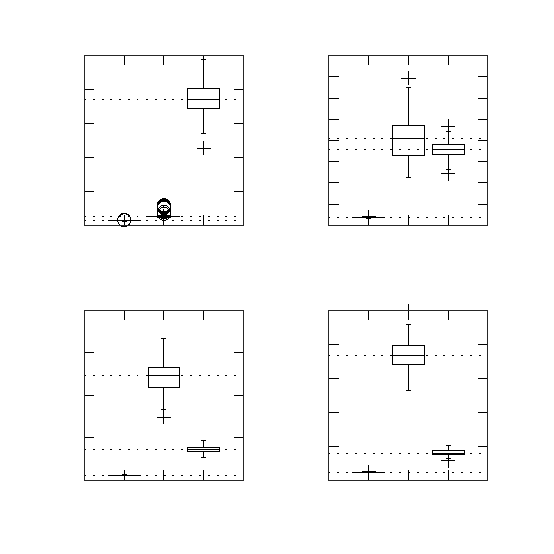
\includegraphics{./figures/experiments/boxplot_errors_CSM_KUF_NDT_sm0}}%
    \gplfronttext
  \end{picture}%
\endgroup

  \caption{\small Pose errors of FSMSM, CSM, and NDT for maximal uniform
           position displacements $\delta_{xy} \in U_{xy}(-0.20, +0.20)$ m and
           maximal uniform orientation displacements
           $\delta_\theta \in U_\theta (-\pi / 4, + \pi /4)$ rad for
           $\sigma_{\bm{M}} = 0.0$ m over $E = 100$ runs per noise level tested
           $\sigma_R$}
  \label{fig:errors_sm0}
\end{figure}


